\begin{figure}
\centering
\begin{subfigure}[t]{0.3\textwidth}
\centering
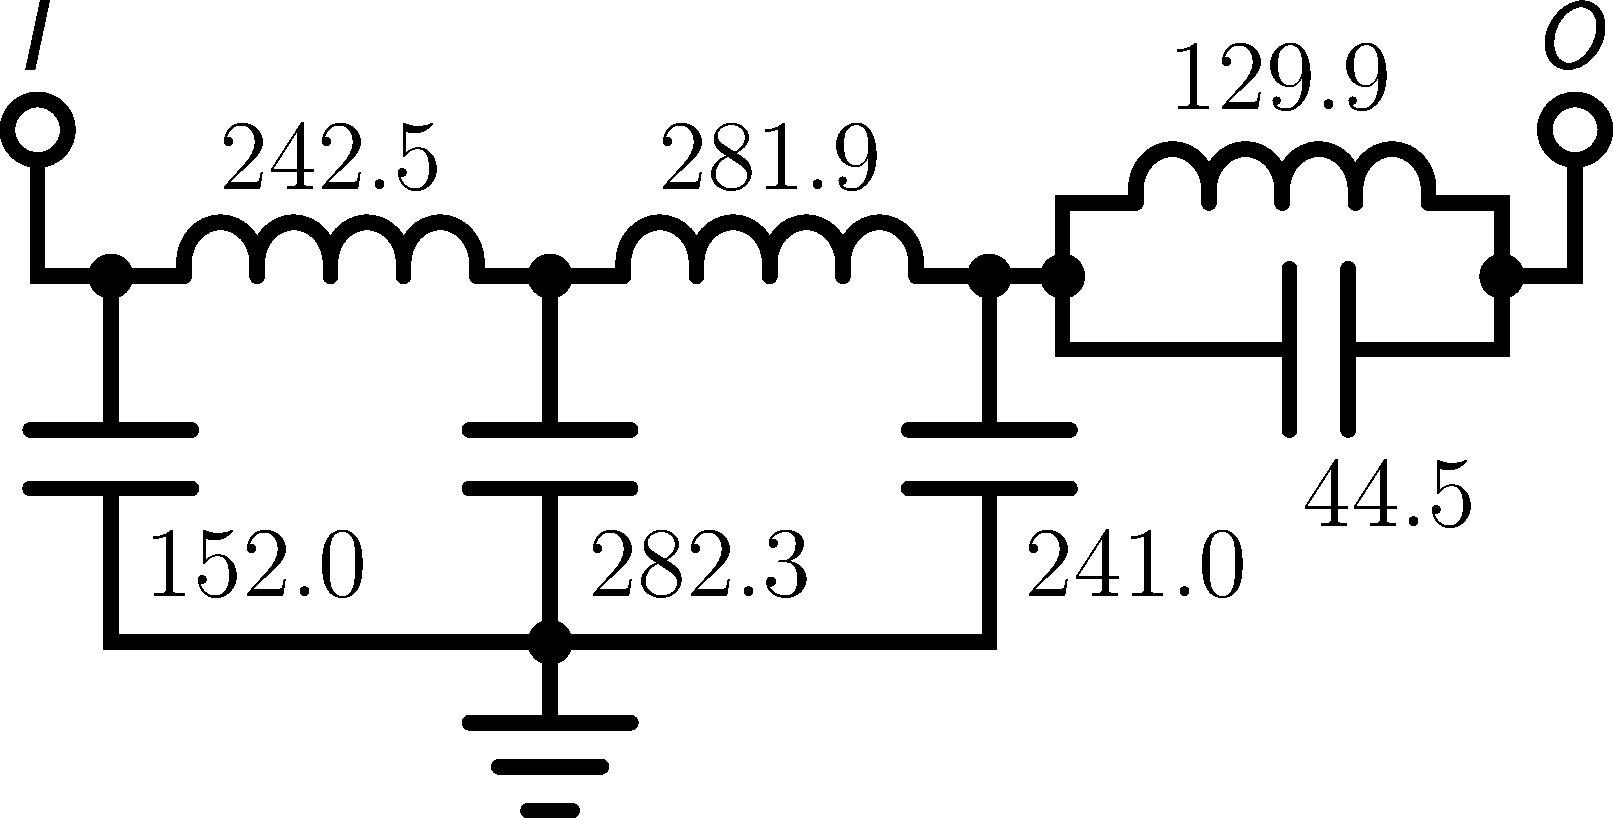
\includegraphics[scale = 0.14]{../ch6/figures/lpf4_circuit1}
\caption{$\{0.0875, 63.08\}$.\label{fig:lpf4_circuita}}
\end{subfigure}%
\begin{subfigure}[t]{0.3\textwidth}
\centering
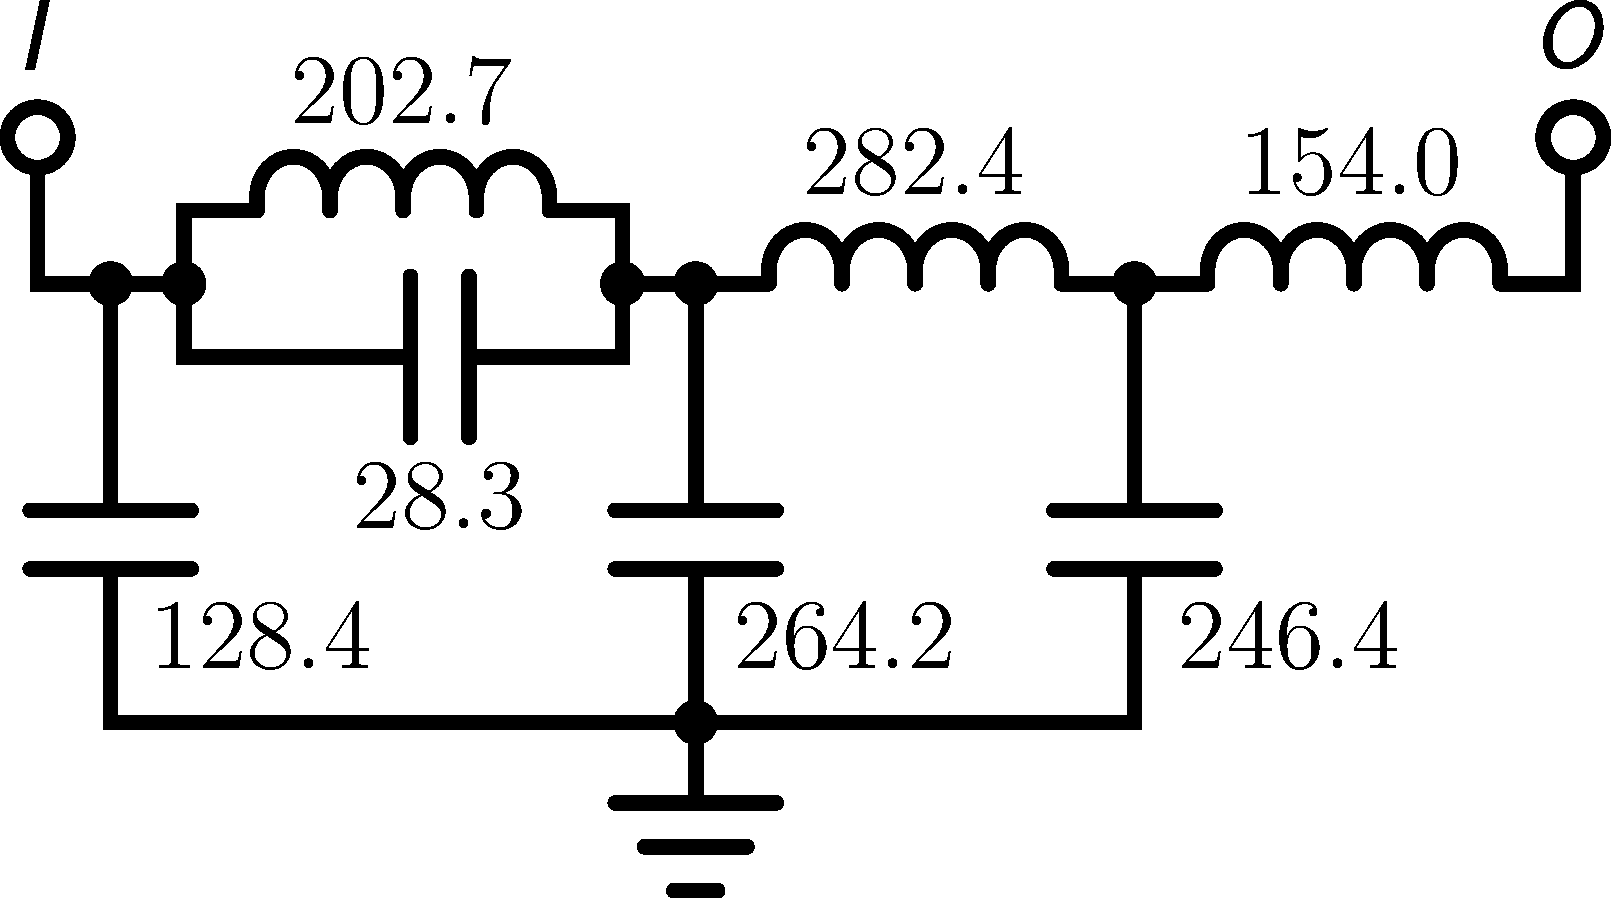
\includegraphics[scale = 0.14]{../ch6/figures/lpf4_circuit2}
\caption{$\{0.1222, 62.92\}$.\label{fig:lpf4_circuitb}}
\end{subfigure}%

\caption[Top two closest to be feasible circuits for \nameref{sec:ch6:lpf} task \#4.]{Top two closest to be feasible circuits for \nameref{sec:ch6:lpf} task \#4 and realized gains $\{K_p,K_s\}$ with respect to $f_p=1000$ Hz and $f_s=2000$ Hz (units are mH and nF).\label{fig:lpf4}}

\end{figure}